

\chapter{Literature review}
This chapter focuses on the information and research materials that were gathered and used in the making of this thesis. The chapter explores computer vision and its techniques, followed by the reasoning behind the chosen object detection for edge devices. Lastly, the chapter explains the use of transfer learning and data augmentation for training neural networks with limited resources.

\section{Previous works}
The internet is brimming with applications designed to enhance board games with computer vision on smartphones. Previous works by Grossmann \cite{grossman} and Hurta \cite{hurta} both implemented applications enhancing the game \textit{Krycí Jména}, or Codenames in english. Both of these works utilized text recognition to read cards and help players or provide additional computer players to play with. Another work by Široký \cite{siroky} in 2021 focused on \textit{Checkers, Gomoku and Nine men’s morris} which utilizes classical computer vision instead of CNNs. More recent work by Takács \cite{takacs} from 2024 implemented an Android mobile library for so called \textit{smart assistants}, applications on mobile devices that help with playing board games, similarly to this thesis.  

As mentioned before, the internet is full of similar works, as all of the previously mentioned examples are from the same institution, Brno University of Technology.

% ===========================================================================================

% ===========================================================================================


\section{Computer Vision}
\label{ComputerVision}
Computer vision is a subfield of artificial intelligence, and it aims to equip machines with the ability to perform visual tasks of recognizing and processing image data \cite{computerVisionIBM}. To us humans, this is something we don't even think about. However, the process of recognizing objects based on their geometry, color, and size is more complicated than we might think. In recent years, this field has become rather popular even outside of academic grounds, mostly thanks to autonomous cars, personal AI assistants, or even in the medical field \cite{computerVisionNX}.

\subsection{Object recognition tasks}
As the research continued, the field widened, and so did the different techniques of computer vision, all in pursuit of general \textbf{object recognition} \cite{computerVisionIBM}.

\textbf{Image classification} is the simplest form of the general object recognition task, which is the goal of computer vision. It classifies the image as a whole into predefined classes and gives it the most probable label.

\textbf{Object detection} is a further expansion of image classification; it combines object localization and image classification into one. It results in a list of coordinates or regions containing certain objects, along with the confidence score for these objects. These coordinates are usually in the form of rectangles and contain x and y coordinates along with the width and height. These so called bounding boxes represent detected objects in the image.

\textbf{Image segmentation} advances object detection, and instead of creating bounding boxes, it uses a pixel-level version of object detection. It groups parts of the images into segments, which are then labeled.

\subsection{Convolutional neural network and transformer based models}

Computer vision as a research field started in the last century. As stated in \cite{computerVisionNX}, one of the first articles \cite{mcculloch1943logical} was released in 1943, in which the researchers attempted to model artificial neurons based on biological ones. This laid the groundwork for the neural networks as we know them today. The next great leap was achieved in 2001 by Viola \cite{viola}, who introduced a rapid object detection system capable of detecting facial features in real-time. A decade later, in 2012, Krizhevsky \cite{krizhevsky} made another significant leap by training a deep convolutional neural network on a large dataset containing 1.2 million image samples and winning an ImageNet LSVRC-2010 contest. This changed computer vision and shifted towards using \textbf{convolutional neural networks} (hereinafter referred to as CNN) instead of traditional computer vision techniques with handcrafted feature extraction. 

A more recent trend uses \textbf{Foundation models} built utilizing \textbf{Transformer} architecture instead of CNN. Foundation models are trained on large scale datasets, often using self-supervised learning, which allows them to learn general representations from data. This allows them to be tailored to specific tasks such as object recognition. The \textbf{Transformer} architecture, often used by these models, was proposed by Vaswani \cite{vaswani2017attention} in 2017. This approach enabled new methods for performing object recognition tasks, such as Segment Anything Models (SAM3) and Distillation of knowledge with No labels v2 (DINOv2).

% ===========================================================================================

% ===========================================================================================

\section{Object detection on edge devices}
Mobile devices, referred to as edge devices in computer vision, still lack the raw computational power compared to the most powerful GPUs available for personal use or data centers. Even though edge devices are not the most powerful, the convenience of a computer vision capable device right in your pocket is desired. Because of that, a contest for edge devices was first held in 2015 named Low-Power Image Recognition Challenge (LPIRC) \cite{alyamkin2019low}.

Therefore, it is necessary to choose an architecture providing the best performance while achieving the best possible precision. A recent study shows that transformer based architectures are catching up to CNN based architectures \cite{wang2026evolution}. However, based on the results, a CNN based architecture called You Only Look Once (YOLO) was chosen due to its more mature architecture and better performance. Similar results can be observed in older surveys comparing CNN architectures \cite{objectDetectionSurvey2024, objectDetectionSurvey2025}.

\subsection{YOLO - You Only Look Once}
\label{yolo}
In 2016, a Redmon presented a new single shot architecture called YOLO \cite{Redmon_2016_CVPR}. Other approaches, like R-CNN introduced in 2014 \cite{girshick2014rich}, search the image for possible bounding boxes and then run classifiers on those parts of the image, which are also called two stage classifiers. YOLO uses a single CNN, predicting both bounding boxes and confidence scores in one step. This approach makes YOLO fast in comparison with, up to that point in time, state-of-the art two stage CNNs. It also provides more context, as the model sees the image as a whole, unlike R-CNN, which uses a sliding window, which results in networks lacking context about the entire image.

% ===========================================================================================

% ===========================================================================================

\section{Transfer learning and pretrained models}
\label{pretrainedModels}
\label{transferLearning}
Neural networks are composed of layers. These layers are made of neurons with different weights assigned to them. The optimization of weights via backpropagation in neurons is what we call training in computer vision. Training neural networks changes their \textit{"response"} to input data (in this case, image data). This process results in neural networks progressively learning how to recognize features, which leads to the capability to detect objects.

Layers of neural networks can be grouped or separated into parts. Using YOLOv8 as an example, it is made up of a \textbf{backbone} and a \textbf{head}. Freezing the backbone part of the network and retraining the head for a specific task is called \textbf{transfer learning}. 

A very simplified example of this would be using a neural network that can distinguish geometric objects and retrain it to detect composite objects, such as eyeglasses composed of two circles and a connecting line. In this case, the first neural network, used as a backbone, understands what circles are but does not understand the concept of glasses. The newly trained head utilizes the knowledge from the backbone and learns to recognize the glasses.

Pandilova, in 2024 \cite{pandilova2024transfer}, demonstrated the use of this technique to boost the performance of the YOLOv8 object detection model. The study demonstrates that using the pretrained backbone of YOLOv8 and training it for a specific task gave it an advantage compared to the original model.

Another advantage of \textbf{transfer learning}, and for this thesis a more crucial one, is its ability to allow developers with limited computational resources to avoid training neural networks on large datasets, such as \textbf{ImageNet} or \textbf{COCO}, which contain hundreds of thousands of labeled images. Training these neural networks may be impractical on common consumer hardware. Instead, they can utilize already existing models and fine-tune them to fit their needs. These pretrained models already understand basic concepts of object detection, such as distinguishing between the background and objects, along with edge detection. Therefore, retraining models for specific use-cases, in this case board game objects, decreases the time and data needed to train these game-ready models. Another example, a model already recognizes playing cards or chess pieces in general. However, retraining the neural network will allow it to distinguish between different types of cards for specific games or individual chess pieces with more exotic designs, such as the ones from the Harry Potter film series.

% ===========================================================================================

% ===========================================================================================


\section{Data augmentation}
\label{dataAugmentation}
Deep neural networks, specifically convolutional neural networks, need data for training the models. Larger datasets result in more accurate neural networks, which is a generally accepted fact \cite{dataAugmentation2}. However, training sophisticated models with limited data might result in insufficient accuracy or \textbf{overfitting} \cite{dataAugmentation1}. This phenomenon occurs when the training loss of the model declines with the number of epochs; however, the validation loss does not decline but rises. Once these two values start diverging from one another, overfitting occurs.

\begin{figure}[hbt]
	\centering
	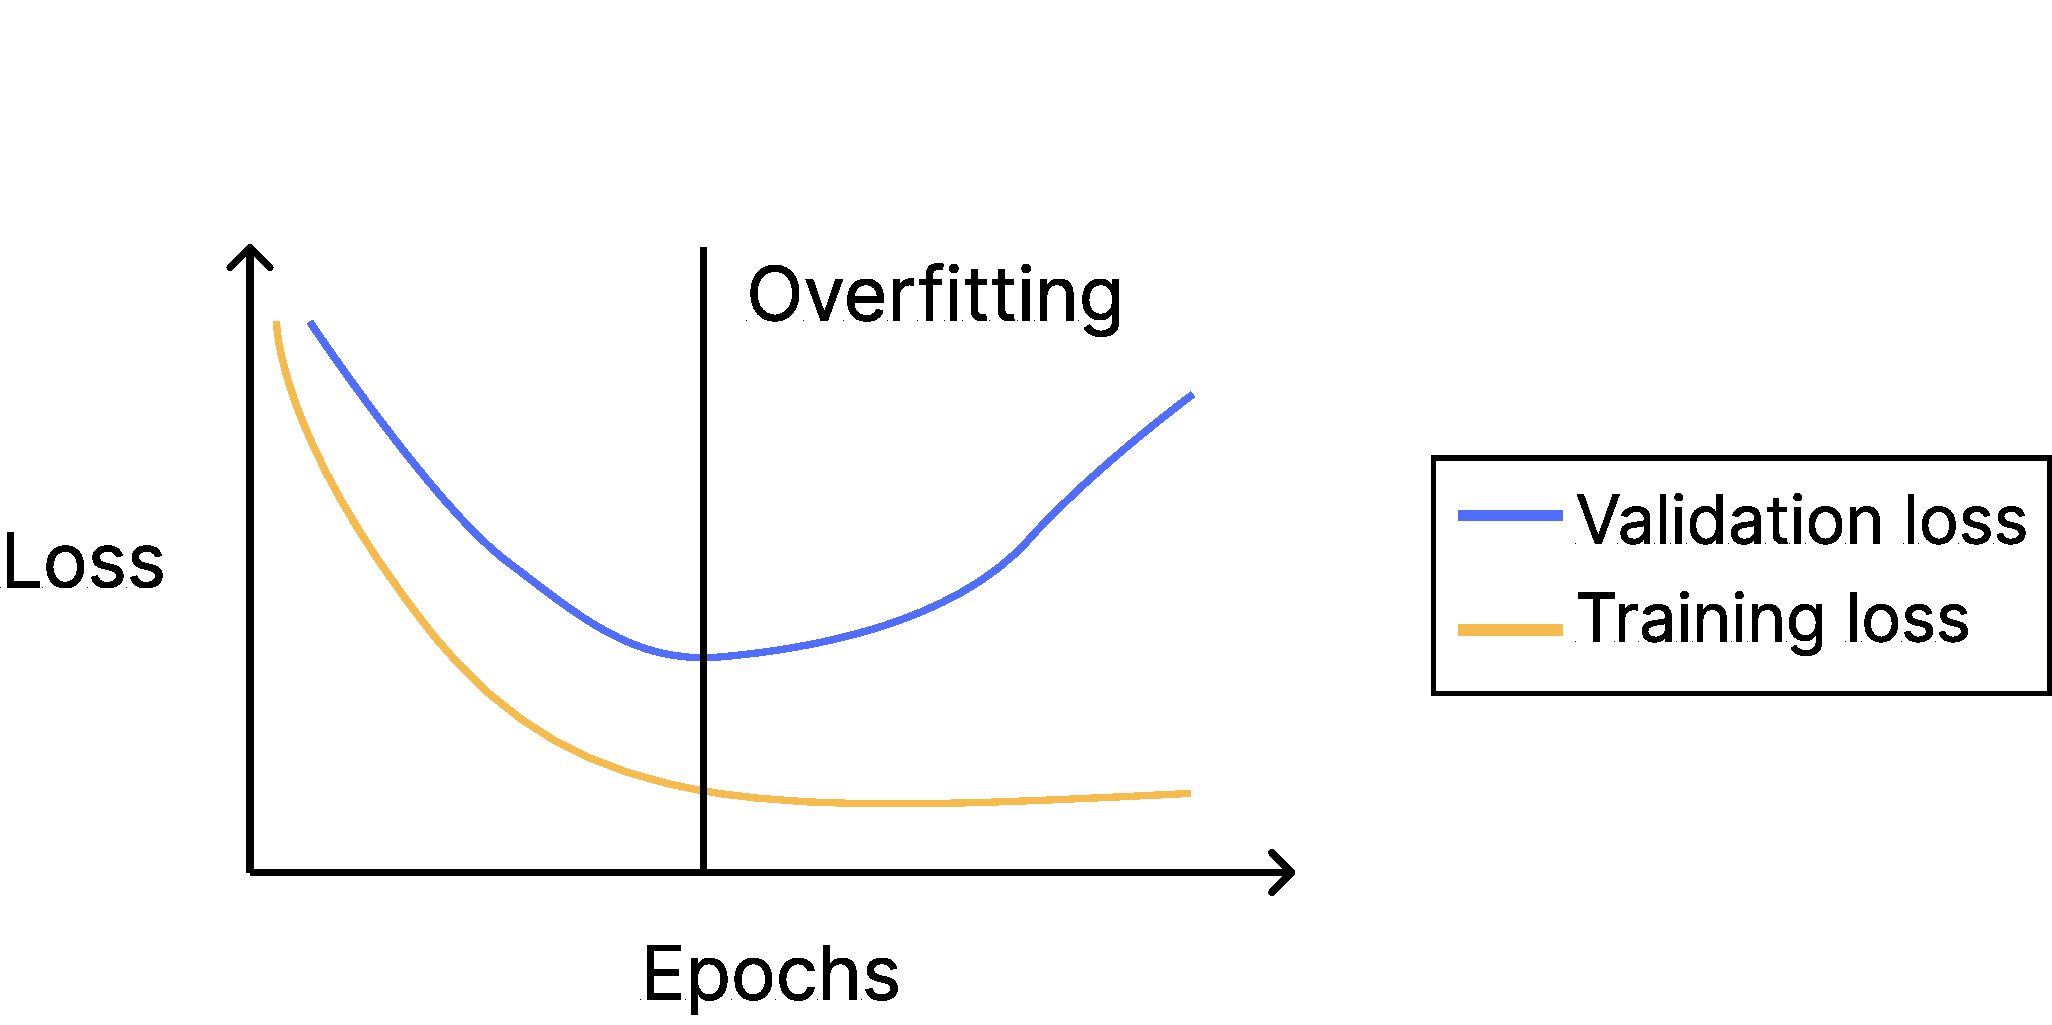
\includegraphics[width=0.6\textwidth]{obrazky-figures/overfitting.pdf}
	\caption[Overfitting illustrative graph]{An illustration of overfitting. Obtained from \cite{dataAugmentation1} and remade into PDF format for lossless scaling}
	\label{overfitting}
\end{figure}

Overfitting can be addressed by obtaining more training data. However, obtaining data for medical, niche, or generally difficult fields is not always a viable option. 

\textbf{Data augmentation} solves this problem by creating artificial/synthetic data. These can be created using traditional and deep learning/generative methods. This thesis focuses on traditional methods, such as changing the brightness or colors of the image. An example of this would be creating a copy of each data sample and decreasing its brightness, which may help the model perform better in dark conditions. Specific implemented data augmentation techniques are discussed in \ref{syntheticDataGeneration}.

% ===========================================================================================

% ===========================================================================================
